%!TEX root = ../PhDthesis.tex
\chapter{Long-range interactions in the visual cortex}

%% jbednar: would be good to add a more recent citation or two to this
%% list, as the newest is 14 years old.
Patchy long-range lateral connections that link regions with similar
visual preferences are one of the most intriguing features of the
early visual cortex. These connections have been suggested to drive a
wide range of contextual-modulation effects including pop-out,
iso-orientation suppression, contour completion, and more
\citep{Gilbert1983, Hirsch1991, McGuire1991, Grinvald1994,
  Fitzpatrick2000, Hupe2001, Stettler2002}. The most commonly reported
effects particularly at high contrast are suppressive, and even though
the connections are known to be excitatory and to primarily target
other excitatory cells, some connections target local inhibitory
neurons that provide strong di- or poly-synaptic inhibition
\citep{Hirsch1991,Weliky1995}.  While both the SCAL and SEPI models
optionally support long-range excitation that could provide such
suppression di-synaptically via the PV inhibitory cells, the
suppression would not be specific for features like orientation,
because the PV cell population is so weakly tuned.

On theoretical grounds, it has been hypothesized that the neural code
in the cortex achieves a sparse representation of the input by
eliminating redundancy \citep{barlow:comneuron89,Olshausen1996}.
Indeed, modulation from the non-classical receptive field has been
shown to suppress redundant information in the input, sparsifying the
representation \citep{Vinje2000}. Here it is crucial that the target
of the suppression is \emph{redundant} activity; achieving sparsity by
simply globally or randomly reducing activity will increase sparseness
but lose information.  For instance, in previous developmental models
of V1 with long-range lateral inhibition, it was shown that both
isotropic and feature-specific connections could achieve a given level
of sparsity, but the isotropic connections did so by reducing
information about the input patterns \citep{Miikkulainen2005}.  For
instance, if two unrelated contours are nearby in an image, isotropic
suppression will eliminate the representation of the weaker one,
achieving sparsity by losing information about the input, while
feature-specific will reduce the number of neurons responding to each
contour separately.

These considerations suggest a difference between short-range
interactions, where the cortex is trying to ensure it achieves maximal
coverage of the feature space, and long-range interactions, where the
neuron is competing to represent the stimulus efficiently, i.e., by
using a sparse code. In the previous models, PV inhibition drove the
local competition, resulting in a smooth coverage of the visual space
with orientation feature detectors, forming an orientation map. Since
the PV neurons act over a local range and are not highly tuned in the
orientation domain, they are generally isotropic in the spatial
distribution and large enough to cover neurons with a wide range of
feature preferences, and thus cannot mediate feature-specific
modulation.

Interestingly, the next-most-common type of inhibitory interneurons
has properties that do seem suitable for mediating specific
modulation.  The Somatostatin immunoreactive (Sst) neurons
\citep{Gonchar2007,Xu2010} are more numerous in layer 2/3, where the
longest-range patchy connectivity is found, and they seem to respond
strongly only under strong, sustained stimulation \citep{Ma2011} or
for very large stimuli \citep{Adesnik2012}. Additionally, their input
scaling does not seem to be linear, with an accelerating response
function driving much stronger responses when recruited consistently
and robustly (as they would be for large or high contrast stimuli;
\citealt{Beierlein2003,Bartley2008,Tan2008}).

On the basis of what we have learned about the PV population from the
previous models and what we know about Somatostatin neurons from the
literature, we therefore propose a general theory of how the circuit
performs specific computations. Afferent input provides strong,
low-latency excitation to the Pv-ir neurons in the thalamocortical
recipient layer 4, which in turn act as both a feedforward inhibition
and dynamic gain control mechanism on the broadly activated excitatory
cell population. This process results in medium-range decorrelation of
the neural activity, which allows short-range recurrent excitation to
amplify the activity in a local column.  The smooth local blobs of
activity that emerge as the response settles then lead to the
formation of a well-organized orientation map.

At the same time, Sst-ir neurons begin to integrate the local activity
through the local and long-range orientation-specific lateral
connections. If their inputs are sufficiently strong they will
activate strongly, allowing this polysynaptic circuit to reduce
long-range correlation in the input activity, further reducing
redundancy. If they are only weakly activated, as would occur when
presented with low-contrast or very sparse input patterns, long-range
lateral excitatory connections are not outcompeted and the circuit can
fill in weak or missing information based on past statistics. In such
a regime, the differential recruitment of the two separate inhibitory
populations would be responsible for a shift in cortical state from a
mode of redundancy-reduction and feature discrimination to one of
visual inference and feature completion.  Note that because Hebbian
learning is proportional to the activity levels, strong inputs should
dominate the learning process, avoiding having the network learn
significantly from the filled-in activations typical of responses to
weak inputs.

In this chapter we extend the SEPI model by adding this second
population of inhibitory neurons modeled after the Sst interneuron
population. In doing so we will demonstrate how this second population
modulates responses to large and high-contrast stimuli, providing
feature-specific inhibition under those conditions, while only very
weakly responding in low contrast conditions. This circuit provides a
considerable advance over previous models of surround modulation,
which typically hard-code the statistical relationships encoded in the
lateral connections while explaining contrast-dependent changes
through a higher inhibitory threshold that conflicts with the
experimental evidence \citep{Li2002, Schwabe2006}. In this model, the
contextual-modulation effects are an emergent phenomenon, arising
directly from the correlations present in the training patterns (as
transformed subcortically).  Identifying and understanding the
circuits involved in these processes is a fundamental challenge for
neuroscience, and will hugely contribute to extending our knowledge of
cortical information processing.

\section{Methods}

In this section we will first introduce the organization and equations
describing the LESPI model and then describe various measurements to
apply to the model to characterize surround modulation effects.

\subsection{The LESPI model}

The \textbf{L}ong-\textbf{R}ange \textbf{E}xcitation, \textbf{S}st,
and \textbf{PV} \textbf{I}nhibition (LESPI) model again builds on the
previous models, this time introducing an additional population of
inhibitory neurons.  These neurons receive no direct afferent input,
being entirely recurrently driven via short- and long-range
projections from the two other V1 cell types. The diagram in
Figure~\ref{LESPIDiagram} shows how the three populations of V1
neurons are connected.

\begin{figure}
	\centering
        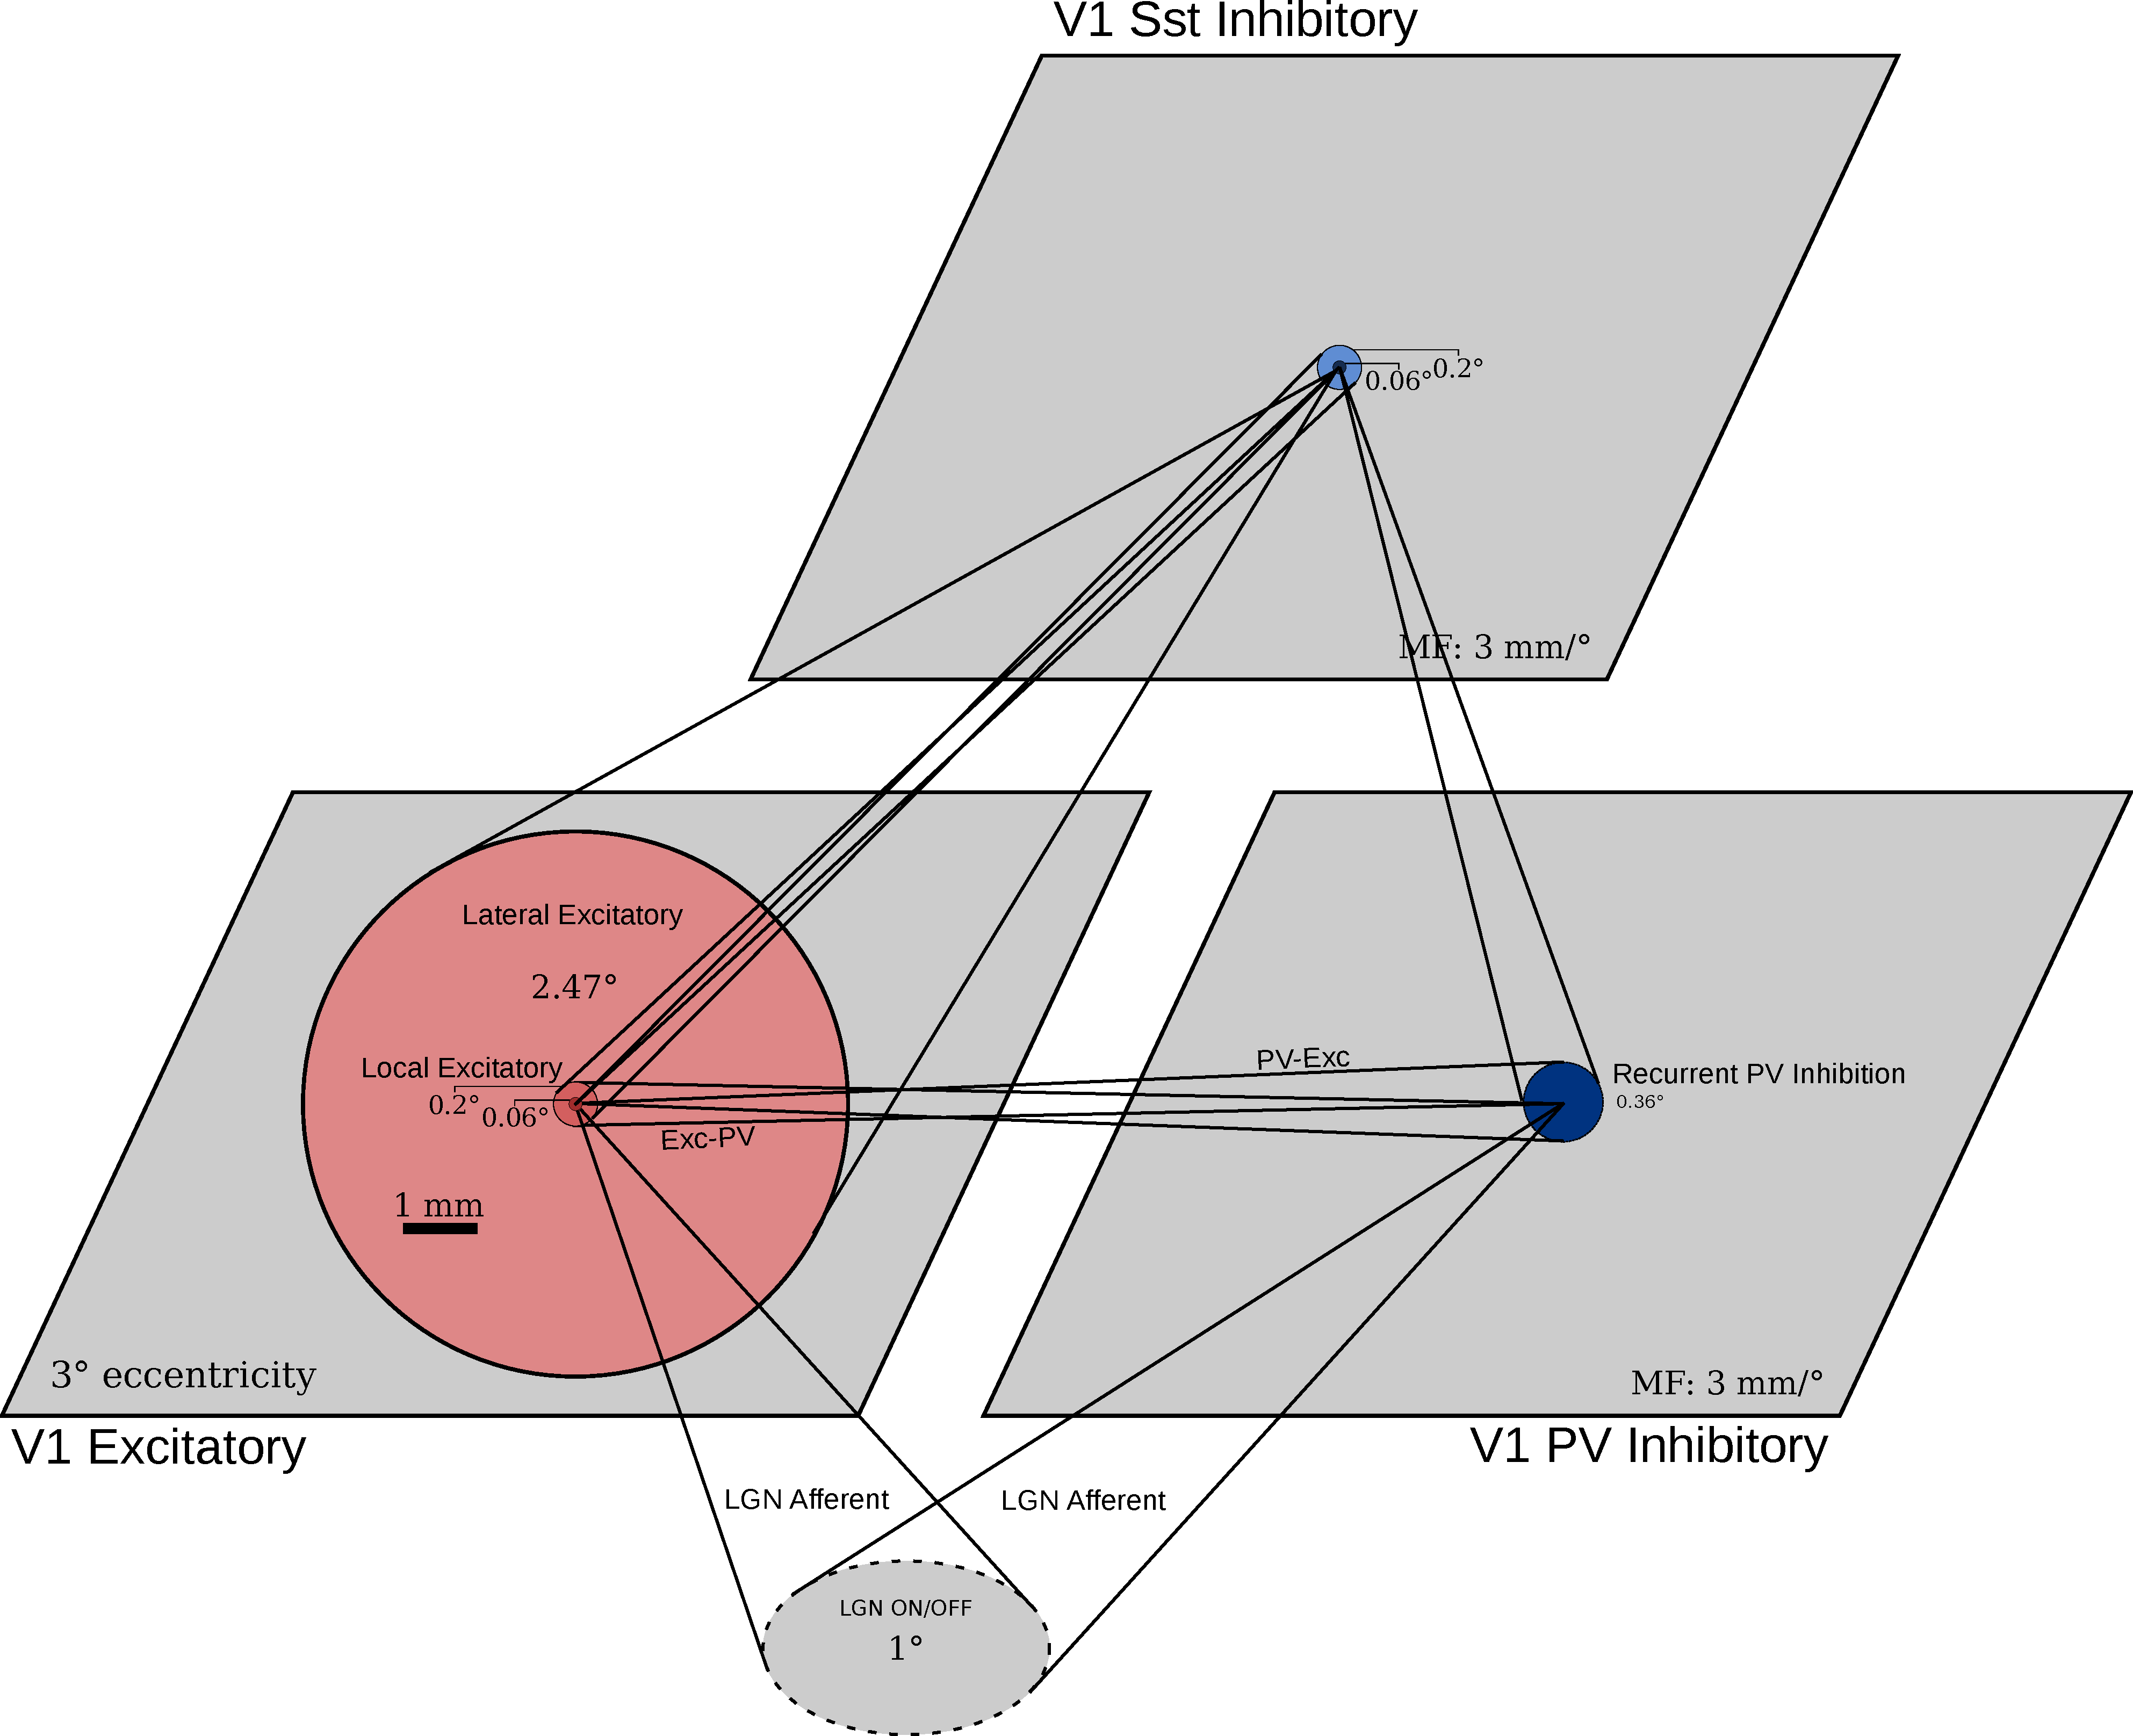
\includegraphics[width=1.0\textwidth]{LESPI_Diagram.pdf}
	\caption{Diagram of the LESPI V1 stage of the model showing the
      spatial scales of the various excitatory (red) and inhibitory
      (blue) connections. Saturated colors indicate the kernel radii,
      while lightly shaded regions indicate kernel cut-off extents.}
        %% jbednar: I can't see which are lightly shaded and which are saturated
	\label{LESPIDiagram}
\end{figure}

The newly introduced Sst population differs from the PV population in
several important respects. First of all, it receives no afferent
connections from the LGN, as this population is most numerous in the
supra-granular layers, which do not typically receive direct afferent
input. Secondly, this population has a much more restricted spatial
profile, being not nearly as extensive laterally as the PV-expressing
basket cells. Most importantly, however, to model the facilitating
response properties of lateral synaptic connections contacting this
population, the model Sst neurons have an exponential non-linearity in
their response. This property allows Sst neurons to activate weakly in
low-contrast conditions, while providing strong suppression when the
input is strong or dense enough. Finally, to model the more sluggish
responses typical of Sst neurons, a hysteresis term is added. In this
way this population will respond strongly after sustained and strong
local and long-range stimulation.

The full set of parameters for the SEPI model are listed in Appendix
\ref{Appendix:Parameters}.

\subsubsection*{Excitatory Activation}

The activity of the excitatory population is computed from all of the
incoming projections, with the Sst population acting as a
multiplicative factor modulating the response of the excitatory
neurons:
%%
\begin{equation}
  \eta_{E} = \frac{\eta_{A} + \eta_{L}}{1 + \eta_{P}} \eta_{SM}
\end{equation}
%%
where $\eta_{A}$ is the LGN afferent activity, $\eta_{L}$ the local
excitatory contribution, $\eta_{P}$ the PV inhibitory contribution,
and the surround-modulation term $\eta_{SM}$ is defined as:
%%
\begin{equation}
  \eta_{SM} = 1 + \eta_{HE} - \eta_{S}
\end{equation}
%%
where $\eta_{H}$ represents the long-range horizontal excitatory
contribution and $\eta_{S}$ is the Sst inhibitory contribution.  In
the standard SEPI model the $\eta_{SM}$ term simply reduces to 1,
eliminating all long-range interactions, while in the long-range SEPI
model $\eta_{SM} = 1 + \eta_{HE}$, with only long-range excitation.
Here LESPI's surround-modulation term provides gain when excitation
exceeds inhibition, and shunting inhibition when the reverse is true.

\subsubsection*{Inhibitory Sst Activation}

The activation of the inhibitory Sst population is given simply by the
summation of the local and lateral excitatory projection activity:
%%
\begin{equation}
  \eta_{S} = \eta_{L} + \eta_{HE}
\end{equation}
%%
The $\eta_{HE}$ term also has hysteresis and an
exponential activation function applied to it, such that its
contribution is given by:
%%
\begin{equation}
  \eta_{HE} (t + \delta\eta) = (\eta(t) + \tau \big[ \eta(t+\delta\eta) - \eta(t) \big])^\beta
\end{equation}
%%
where $\tau=0.2$ and $\beta=3$. This combination of hysteresis and an
exponential non-linearity allows the lateral connections to integrate
over time, accelerating its response under strong and prolonged
activation, which closely models what has been observed in experiments
\citep{Beierlein2003,Bartley2008,Tan2008}.

\subsubsection*{Mechanisms}

The mathematical effect of long-range horizontal connections is
controversial and complex.  The connections typically target distal
dendrites rather than the soma, which would suggest a subtractive
model.  However, there is evidence for multiplicative effects as well
\citep{Wilson2012}, including strong voltage dependence
\citep{Hirsch1991}.  The connections may act multiplicatively by
locally gating excitatory horizontal and feedback inputs at the
dendrites \citep{Ma2011, Gentet2012}. Theoretical studies also suggest
that active dendritic spike backpropagation can lead to multiplicative
increases in gain, while reduction in spike backpropagation can lead
to divisive scaling of the firing rate \citep{Mehaffey2005}. Modeling
the net effect of long-range input as a single multiplicative term,
which can act divisively given sufficient inhibitory input, therefore
provides a convenient but highly simplified abstraction of long-range
interactions.

The overall operation of this circuit can be summarized by the
schematic in Figure~\ref{circuit_diagram}. The diagram shows the
preferential linking of columns with similar orientation preference
via patchy long-range connections and the long-range integration of
Sst neurons, which receive both local and lateral input from pyramidal
neurons, providing di-synaptic inhibition to the local
region. Furthermore it suggests that under low-contrast conditions the
Sst population is effectively disabled, activating only under high
contrast input.

\begin{figure}
	\centering
	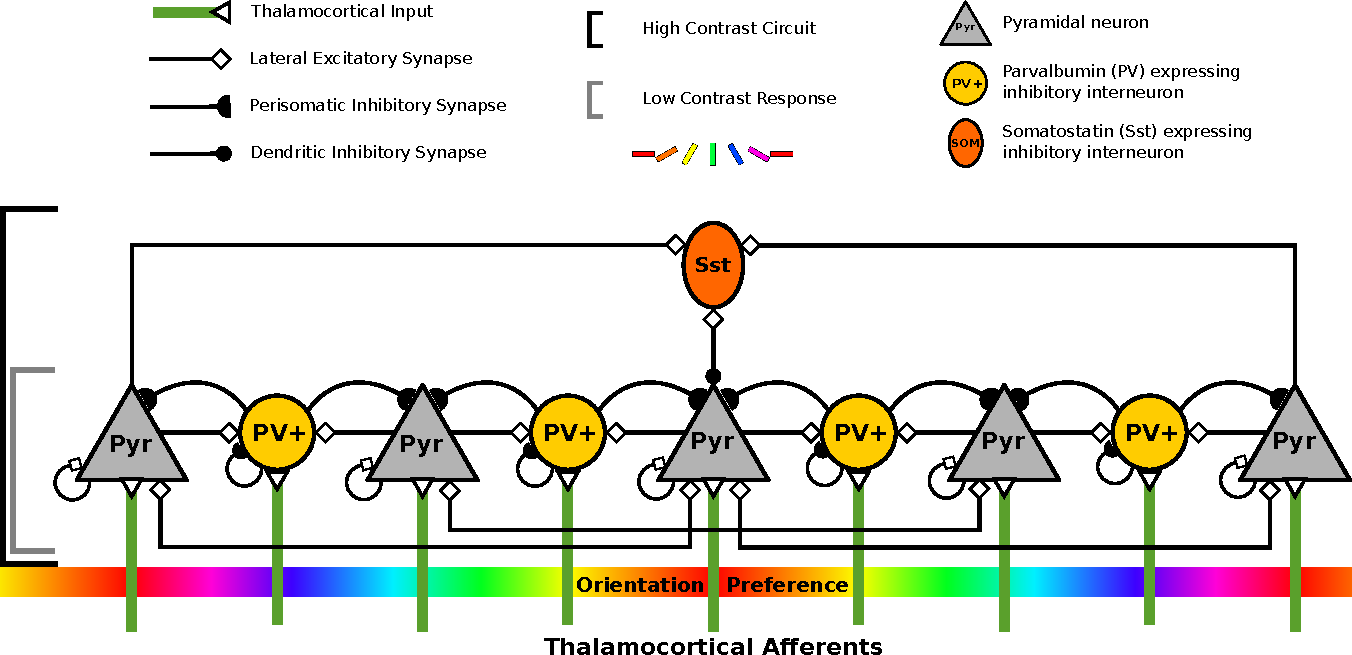
\includegraphics[width=1.0\textwidth]{./v1circuit.pdf}
	\caption[High-level circuit diagram of the LESPI
      model.]{High-level circuit diagram of the LESPI model. The
      schematic represents multiple hypercolumns varying smoothly in
      their orientation preference. PV neurons provide feedforward and
      recurrent inhibition to neurons in the local region,
      regardless of their orientation tuning. Long-range excitatory
      connections link pyramidal cells with similar orientation
      preference, while the Sst population integrates both local and
      long-range input to provide tuned orientation suppression under
      high-contrast input.}
    \label{circuit_diagram}
\end{figure}

\subsubsection*{Sparsity}

In the current form of the model, both afferent and lateral connection
fields are simulated as dense projections of weights in a local
region. However, real lateral connections only form patchy connections
in the cortex. Having these diffuse connections means that only a
fraction of the synaptic weight is concentrated at the patchy
terminals. Informally, we have confirmed that the model self-organizes
well using a simple sparse sprouting-and-retraction algorithm, but
this sparsification algorithm would need to be documented, explained,
analyzed, and validated separately before being applied here. Since
that complexity would be distracting for our current modeling goals,
we instead train the model with dense projections and then
subsequently sparsify it by thresholding all weights below the 90th
percentile. As shown in the results section below, this process leaves
only patchy connections that strongly resemble experimental plots of
patchy long-range connections in layer 2/3 of macaque and tree shrew,
extending up to 4 hypercolumns from the neuron.

Sparsifying the weights in this way has the potential to alter the
activity but since the connections mostly have a modulatory influence
this does not significantly change network responses especially in the
initial response. However influences on the overall tuning and
therefore the map structure cannot be ruled out. To eliminate these
issues future work should therefore pursue an approach that employs
connection sparsity from the start.

\subsection{Visual statistics}

In the models simulated in previous chapters, we have largely ignored
the effect of visual statistics, instead using only simple artificial
training patterns like 2D Gaussians that are always brighter than the
background.  These patterns were used because the models develop
simple cells, strongly tuned for spatial phase.  Patterns like natural
images have a variety of spatial phases, such as light areas
surrounded by dark and dark areas surrounded by light.  When given
such patterns, SCAL or SEPI simple cells with opposite phase
preferences (swapping ON for OFF excitation) will be anticorrelated
and thus far from each other on the cortical surface, disrupting the
maps for orientation and retinotopy \citep{Miikkulainen2005}.  In
contrast, animal maps in the superficial layers used in imaging
studies typically contain complex cells not highly selective for
phase, which modeling suggests will lead them to develop smooth
representations for orientation and retinotopy regardless of the
training patterns \citep{Antolik2010}.

To study contextual modulation, in this chapter we will need to use
input patterns that have long-range correlations, instead of localized
2D Gaussians confined to the width of a receptive
field.  Otherwise, no long-range connectivity will develop by Hebbian
learning.  We will test the effects of a variety of natural image
datasets as well as synthetic stimuli that include long-range
correlations, while bearing in mind that the map patterns when trained
on natural images should not be expected to closely follow results
from animals, due to the phase dependence.  Future versions of the
model can include complex cells to remove this restriction, at a cost
of greatly increased computational and memory requirements and
additional parameters \citep{Antolik2010}. 

\subsubsection*{Natural stimuli}

The visual statistics in different natural stimuli can vary
considerably.  For instance, man-made objects often have very
different statistics from natural objects. Visual scenes in nature
typically contain smoothly varying somewhat circular contours, while
man-made objects exhibit more straight and perpendicular lines
\citep{Perrinet2015}. Experiments suggest that humans can rapidly
classify images of animals and non-animals based solely on the
co-occurence statistics of visual contour elements in the image
\citep{Serre2007, Perrinet2015}. Here we will make use of the various
image datasets used in these studies as training data for the model,
allowing us to compare their effects on contextual modulation.

The image datasets used for these purposes include the target dataset
used by \cite{Serre2007}, consisting of animal images, as well as
multiple datasets obtained by James Bednar in 2010 meant to replicate the
visual experience of a developing animal, both in a laboratory environment,
dominated by high-contrast bars of the animal cages, and a
natural environment dominated mostly by grass, leaves, and trees.

% jbednar: can you change the name ``natural'' to outdoor, if it's A?
\begin{figure}
	\centering
	\includegraphics[width=1.0\textwidth]{./results/lespi/ImagePatterns.pdf}
	\caption[Example image patterns used to train the model] {Example
      image patterns sampled from different image datasets and then
      randomly positioned and rotated. A) Forest and grass taken in
      Gif-sur-Yvette. B) Inside of a tree-shrew cage taken in David
      Fitzpatrick's animal rearing facilities at Duke University.
      C) \cite{Serre2007} target patterns of animals and natural landscapes.}
    \label{image_patterns}
\end{figure}

\subsection{Surround modulation}

To reveal the effects of long-range connections, we will replicate a
series of surround-modulation measurement protocols. In addition to
the simple area-summation-curve measurements described above, we test
two further protocols.  In particular, we are interested in how
stimuli outside the receptive field of a set of neurons can affect
their response, and how those effects vary with contrast. For that
purpose we replicate two measurement protocols, a simple annulus-based
contrast-suppression measurement \citep{Jones2002}, and a protocol
using target and flanker stimuli \citep{Kapadia1995}.

\paragraph{Orientation-contrast suppression}

Orientation-contrast suppression is perhaps one of the most
well-studied surround-modulation paradigms. The measurement involves
presenting a central masked sine grating, optimized to the preferred
size, frequency, and orientation of the neuron being measured. Once
the baseline activity has been measured, an additional surround
annulus with the same frequency is added and varied in contrast, size,
and orientation to measure orientation-dependent interactions between
center and surround (as shown in Figure~\ref{ORC_Stimulus}). In
in-vivo experiments, these measurements are performed using drifting
gratings covering all spatial phases.  Here we are only simulating
simple cells, and so the gratings are optimized for the preferred
phase of each neuron instead.

The center stimulus and the annulus were separated by $0.25^\circ$,
which is smaller than the size of the separation employed by
\cite{Jones2002}, largely because the modeled cortical area is
limited. However the size of the center and surround stimuli were
roughly the same scale with a $1^\circ$ and $3.5^\circ$ diameter
respectively.

\begin{figure}
	\centering
        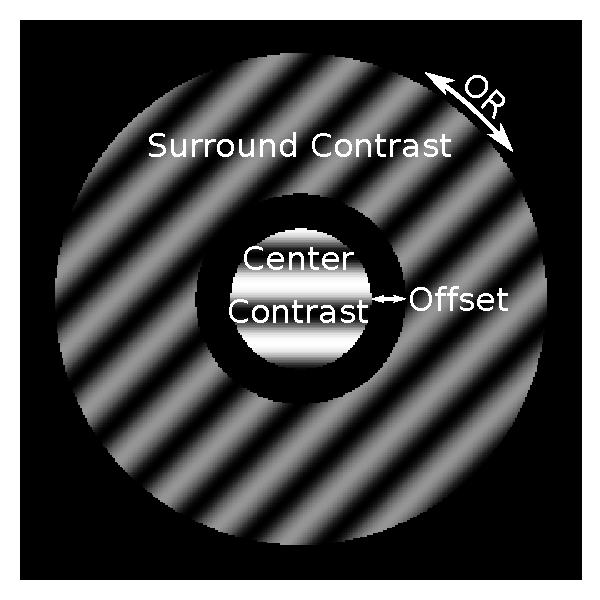
\includegraphics[width=0.5\textwidth]{ORC_Stimulus.pdf}
	\caption{orientation-contrast stimulus measuring modulation by a
      sine grating annulus on the response of a central neuron
      responding to a central sine grating disk of the same spatial frequency.
      Stimulus is varied by center and surround contrast, surround
      orientation and the offset between the central disk and the
      surround annulus.}
	\label{ORC_Stimulus}
\end{figure}

In order to quantitatively assess the orientation-contrast suppression
we used the orientation-contrast suppression index defined as:

\begin{equation}
  OCSI = \frac{R_0 - R_{\frac{\pi}{2}}}{R_0}
\end{equation}

where $R_0$ represents the response at the preferred orientation and
$R_{\frac{\pi}{2}}$ at the orthogonal orientation.

\paragraph{Pop-out}

Another well-studied effect in the surround-modulation
literature is ``pop-out'', where a visual stimulus 
embedded within a number of dissimilar features strongly stands
out. It is thought this effect relies on similar features suppressing
each other, leaving the dissimilar unaffected and therefore
``popping-out`` of the background \citep{Kastner1997}. In order to
test this surround-modulation effect we generate visual patterns
containing a target bar stimulus surrounded by a circle of flanker
stimuli, which are either co-aligned with the target (iso-condition)
or orthogonal to the target (cross-condition).
The response to the targets and the flankers is then computed as the
mean activity of the non-zero responding units with two annuli, one
covering the central 1 degrees and the other covering the remaining
simulated area.

\section{Results}

As previously discussed, the surround-modulation effects in the model
are highly dependent on the statistics of the visual input used for
training. The following analyses all use either the ``natural`` or the
``treeshrew`` (cage) dataset shown in
Figure~\ref{image_patterns}. This is because the Gaussian patterns are
drawn randomly and do not contain any long-range correlations the
model could learn and encode in its lateral connectivity.

Before characterizing the responses to more complex patterns, we will
once again show how the response to a simple Gaussian pattern evolves
over time before and after development, which is shown in
Figure~\ref{LESPIResponse}. When comparing this response to the SCAL
model (see Figure~\ref{SCALResponse}) it is immediately noticeable
that the model exhibits significantly more suppression, which can be
attributed to inhibition from the additional inhibitory population
(having kept the same strength for the first population when the
second was added). Later on we will see that the timecourse of
responses is highly stimulus dependent, resulting from the richer set
of interactions when compared to the SCAL and SEPI models.

\begin{figure}
	\centering
    \includegraphics[width=1.0\textwidth]{./results/lespi/LESPI_Response.pdf}
	\caption[LESPI responses to a simple Gaussian pattern before and
      after self-organization.]{LESPI responses to a simple Gaussian
      pattern before and after self-organization on the natural
      dataset. Top left shows the input pattern and the LGN ON/OFF
      response to the pattern. Top right shows the evolving patterns
      of activity before, during, and after development. The response
      of the central neuron at the different stages of development is
      shown at the bottom. Neurons exhibit strong suppression after
      the initial onset, depending on the stimulus being shown.}
	\label{LESPIResponse}
\end{figure}

Secondly it is important to get an understanding of the map
organization and how that may influences the results. In Figure
\ref{LESPI_ORTuning} an orientation map and the afferent weight
patterns for the simple Gaussians and two natural image datasets is
shown. Visual comparison immediately highlights the disrupted
organization of the orientation map when the model is trained on
natural images. The afferent connection patterns highlight what is
causing this disruption. In the natural image trained models the
afferent connections form a phase map, flipping between ON-center and
OFF-center receptive fields. This is because these patterns are
locally anti-correlated and therefore segregate into separate
regions. Additionally lower spatial frequency preference in the
treeshrew case can be observed, made evident by the two-lobed, rather
than three-lobed receptive fields.

\begin{figure}
	\centering
    \includegraphics[width=1.0\textwidth]{./results/lespi/LESPI_ORTuning.pdf}
	\caption[LESPI model orientation map when trained on Gaussian
      patterns and treeshrew and natural image datasets]{LESPI model
      orientation map when trained on Gaussian patterns and treeshrew
      and natural image datasets. A, B, C) Orientation maps showing
      good organization in the Gaussian case, and phase disrupted
      organization in the treeshrew and natural conditions. D, E, F)
      Afferent connections for the three conditions, highlighting the
      phase organization in the natural condition and spatial
      frequency differences in the treeshrew condition.}
	\label{LESPI_ORTuning}
\end{figure}


\subsection{Orientation contrast suppression}

Orientation-contrast suppression is one of the most well-studied
paradigms in the surround-modulation literature. One of the most
thorough analyses was performed by \cite{Jones2002}, varying the
relative size and offset of the center stimulus and surround annulus.
The measurements were performed in the model trained on the
``natural`` dataset, which does not have as highly biased statistics
as the laboratory datasets.

As a first step, the orientation-contrast curve was measured for a
number of randomly chosen neurons under high-contrast conditions.
Non-responding units were rejected, making up roughly 29\% of the
neurons. This was likely due to imperfect fitting of the optimal
parameters. By normalizing the response and averaging the curves and
computing the standard error, an average contrast suppression curve
was computed and can be seen next to the orientation-tuning
suppression curve from a single neuron measured by \cite{Jones2002} in
Figure \ref{ORTC_Jones}. The result shows that the model neurons have
realistically strong iso-orientation suppression with a well defined
shape, which does not vary considerably in width.

\begin{figure}
	\centering
        \includegraphics[width=1.0\textwidth]{./results/lespi/ORTC_Jones_Comparison.pdf}
	\caption[Averaged orientation-contrast suppression curve compared
      against \cite{Jones2002} example curve.]{Averaged
      orientation-contrast suppression curve compared against
      \cite{Jones2002} example curve. A) Shows the normalized and
      averaged orientation contrast suppression curve from 71 neurons
      against the individual orientation tuning curves of those
      neurons (spread represents standard error). B) A sample
      orientation-contrast suppression curve reproduced from
      \cite{Jones2002}. Results from model trained on natural
      dataset.}
	\label{ORTC_Jones}
\end{figure}

\subsubsection*{Contrast Dependence}

In addition to measuring the classical high-contrast suppression
curve, the equivalent measurement was performed for an individual
neuron under both low and high-contrast conditions. The orientation
contrast tuning curves were measured at each settling step of the
model and are shown in Figure~\ref{ORTC_ContrastDependence}. As these
results clearly show, the neuron exhibits very different effects under
the two conditions. When the local and global contrast is low, the
response of the neuron is enhanced, while high-contrast stimulation
demonstrates the same suppressive effect that is evident in the
averaged suppression curve in Figure~\ref{ORTC_Jones}.

% jbednar: monochrome stimuli would be better here; less pretty but
% more obvious
\begin{figure}
	\centering
        \includegraphics[width=1.0\textwidth]{./results/lespi/ORTC_ContrastDependence.pdf}
	\caption[Dependence of orientation-contrast suppression on local
      and global contrast.]{Dependence of orientation-contrast
      suppression on local and global contrast. A, C) Low- and
      high-contrast orientation-contrast suppression patterns. B, D)
      Corresponding orientation-contrast suppression curves showing
      facilitation at low contrast and suppression at high contrast,
      respectively. Results from model trained on natural dataset.}
	\label{ORTC_ContrastDependence}
\end{figure}

In order to find the cross-over point at which facilitation turns to
suppression, the contrast of both the center and surround pattern was
varied and the OCSI was calculated for different durations. The
corresponding plot is shown in Figure~\ref{ORTC_ContrastCurve},
highlighting again that suppression weakens as the response is
settling, but more importantly clearly shows that the inflection point between
excitation and suppression for this particular neuron lies at about
9\% contrast.

This analysis also demonstrates how the suppression varies over the
time course of the response, beginning shortly after onset (which
occurs after a duration of about 0.25 and is excluded from analysis)
and peaking at around 0.7 before weakening again. Since this model has
not been temporally calibrated, it is hard to relate these times to
experiments. Investigating the precise time-course of the different
cell classes will make it clearer how the contrast dependence of the
surround modulation emerges from the circuit.

\begin{figure}
	\centering
        \includegraphics[width=0.8\textwidth]{./results/lespi/ORTC_CSContrast.pdf}
	\caption[Contrast dependent switch from facilitation to
      suppression.]{The relationship between contrast and orientation
      contrast suppression. A) Effect of varying center and surround
      contrast on the OCSI, demonstrating a shift from facilitation
      (positive OCSI) to suppression (negative OCSI). B) Effect of
      varying center and surround contrast independently, demonstrating
      that both local and surround context influence contextual
      modulation. Results from model trained on natural dataset.}
	\label{ORTC_ContrastCurve}
\end{figure}


\subsubsection*{Timecourse}

In order to get a better understanding of how the different cell
classes and synaptic projections interact to give rise to the
contextual-modulation effects seen above, the timecourse of the
activity can be visualized. The timecourse of the responses under four
different conditions is shown in Figure~\ref{ORTC_TimeCourse}. The
top-row shows the response under low-contrast conditions for the
iso-orientation and cross-orientation condition and highlights how the
iso-orientation facilitation emerges. Comparing A and B it is clear 
how the lateral excitation increases the excitatory response in
the iso-orientation condition but activates more weakly in the
cross-orientation condition. Similarly in the high-contrast case, the
Sst population activates much more strongly in the iso-orientation
condition (C) than in the cross-orientation condition, as expected due
to the feature selectivity of the Sst neurons.

\begin{figure}
	\centering
        \includegraphics[width=1.0\textwidth]{./results/lespi/ORTC_TimeCourse.pdf}
	\caption[Time-course of neural and synaptic projection responses
      under four conditions, demonstrating how a contrast-dependent
      switch between facilitation and suppression occurs]{Time-course
      of neural and synaptic projection responses under four
      conditions, demonstrating how a contrast-dependent switch
      between facilitation and suppression occurs. Visualizes how
      inerneuron activity and lateral excitatory projection affect the
      response of the excitatory projection (in red). A) In the
      low-contrast iso-orientation condition, lateral excitation
      exceeds the activation of the V1 Sst population, resulting in
      facilitation. B) In the low-contrast cross-orientation
      condition, very little surround modulation occurs. C) In the
      high-contrast iso-orientation condition, the Sst population
      activates strongly causing strong suppression. D) Under the
      high-contrast cross-orientation condition, Sst neurons are only
      weakly recruited, resulting in a moderate amount of modulation.
      Results from model trained on natural dataset.}
	\label{ORTC_TimeCourse}
\end{figure}

\subsection{Size tuning}

The effects of both distance and contrast can best be
explained when looking at the size-tuning curves of all three
populations. A representative example of size-tuning curves measured
from all three populations at a single location is shown in
Figure~\ref{LESPI_SizeTuning}. The excitatory neuron shows a
significant shift towards larger size preferences at lower contrast
($>3\times$). This shift is largely driven by the fact that both of
the inhibitory populations demonstrate even more significant shifts in size
tuning. The most striking feature of these results is the very gradual increase
of Sst activation as the stimulus grows at low contrasts. This means
that for very small stimuli the Sst neurons provide very little
inhibition, allowing facilitatory effects to occur.

\begin{figure}
	\centering
        \includegraphics[width=1.0\textwidth]{./results/lespi/LESPI_SizeTuning.pdf}
	\caption[size-tuning curves of the excitatory, PV, and Sst
      population at various contrasts.]{size-tuning curves measured in
      the LESPI model trained on natural stimuli for the A)
      excitatory, B) PV inhibitory, and C) Sst inhibitory
      population. The curves show clear modulation by stimulus
      contrast shifting toward higher size preferences, driven
      primarily by the shifts towards larger maximal suppression at
      low contrasts in the inhibitory populations. Results from model
      trained on natural dataset.}
	\label{LESPI_SizeTuning}
\end{figure}

\subsection{Flanker Modulation}

A second often-used paradigm to measure surround-modulation effects is
presenting a target stimulus optimized for a particular neuron, and
then adding flanker stimuli, which may vary in orientation from the
central neuron. These patterns are much more sparse and therefore do
not engage the circuitry in the same way a natural image or
even a sine grating would. We are particularly interested
whether the surround-suppression effects that were seen above are
sufficient to account for various saliency-based computations that are
thought to originate in the early visual cortex. Specifically, can
iso-orientation suppression drive a pop-out effect where visual
elements with similar orientations suppress each other while
leaving any heterogeneous elements unaffected?

The simplest means of testing this effect is to embed a target bar
stimulus in a ring of iso- or cross-oriented flankers, then compute
the average activity in the region corresponding to the flanker
against the region corresponding to the target. The
effect of this can be seen in Figure~\ref{Flanker_PopOut}, showing the
two stimulus conditions and a plot of the average non-zero response in
the central target region and in an annulus around it corresponding to
the flanker region. The target activity is elevated above both the
flanker activation in the same stimulus condition but more importantly
it is also elevated when compared to the iso-orientation condition
where all flankers have the same orientation.

\begin{figure}
	\centering
        \includegraphics[width=1.0\textwidth]{./results/lespi/Flanker_Popout.pdf}
	\caption[Pop-out effect in simple flanker paradigm.]{Demonstration
      of pop-out when presenting a target along with either
      iso-oriented or cross-oriented flankers, then averaging the
      response in two annuli corresponding to the target and flanker
      region. The V1Exc sheet responses are colored by the
      orientation preference of the neurons, showing that the center
      and surround regions can activate different orientations, and
      that the central response is suppressed by iso-oriented flankers
      but pops out when surrounded by cross-oriented flankers.
      %% jbednar: doesn't there need to be a third case, of no
      %% surround, to say whether it's really pop-out or just lack of
      %% suppression ?
      The average response in the target region in both
      conditions is represented by the solid lines, while the annulus
      region is shown as dotted lines. The averaged responses
      highlight pop-out of the target stimulus from the background in
      the cross-orientation condition, but not the iso-orientation
      condition. Results from model trained on treeshrew dataset.}
	\label{Flanker_PopOut}
\end{figure}

\section{Discussion}

In this chapter we introduced the LESPI model as an extension of the
models presented in previous chapters, demonstrating how the model
will exhibit many of the contextual-modulation effects that are known
to occur in the primary visual cortex. Unlike other
surround-modulation models, this model explains mechanistically how
the long-range patchy excitatory connections emerge in the model, and
how a specific class of inhibitory neurons can explain contrast- and
context-dependent changes in surround modulation.

Using standard experimental paradigms for assessing surround
modulation in the primary visual cortex, we show that long-range
lateral connectivity targeting both excitatory and inhibitory neurons
can provide a good match to electrophysiological and psychophysical
results. The model allows inspecting the responses of every single
neuron, providing comprehensive predictions for how neural responses
are modulated.

\subsection{Feature-dependent modulation}

There are numerous models that have been used to explain
feature-specific surround-modulation effects in the visual
cortex. These models usually start by hardwiring a set of feature
detectors, which are then connected according to their similarity in the
feature space \citep{Li2002, Schwabe2006}. When modeling V1, the models
thus connect neurons with similar orientation preference, to replicate
the orientation-specific patchy connectivity that has been observed
\cite{Bosking1997}. However, while such models
are useful to study specific phenomena, they provide an unsatisfyingly
narrow explanation of cortical function, which does not generalize
across different brain regions and sensory modalities.

Developmental models such as the model presented here explain the
emergence of surround-modulation effects as a consequence of the way
the circuit self-organizes and learns the statistics of the natural
world. In other words, unlike other models, none of the surround
modulation effects are hard-coded. Instead, the effects emerge
naturally due to simple and general mechanisms: Hebbian learning,
divisive gain control, homeostasis, and local microcircuits composed
of various cell types. The emergence of iso-orientation facilitation
and suppression is therefore the result of the model extracting
co-occurrences in the training patterns. Indeed, by comparing models
trained on simple independent Gaussian patterns, with the same model
trained on natural or laboratory images, it is clear that the
long-range modulatory effects only emerge when the training patterns
contain consistent long-range correlations.
%% jbednar: need to actually show that, at the start of this chapter.

These results add to the growing amount of literature suggesting that
the cortex uses the statistical dependencies between sensory features
to optimize neural coding \citep{Vinje2000, Simoncelli2001} and
improve performance in specific tasks \citep{Geisler2001}. In the
LESPI model the long-range connections learn a statistical
distribution of the inputs, and can then modulate the response to give
rise to both facilitatory effects and suppressive effects. These
effects are mediated through a divisive normalization mechanism
similar to those used in models using higher-order correlations to
optimize neural coding by reducing redundancy \citep{Spratling2011,
  Coen2015}. This work suggests that the patchy lateral connections in
primary visual cortex could be the first stage for feature-specific
redundancy reduction, without requiring specific feedback from
higher-level areas. How much the lateral connections actually
contribute to decorrelating activity and influencing development is an
empirical question that will require further investigation, but the
results here show that these connections could account for quite a
range of contextual effects.

At the same time, the spatial scales over which the lateral connections
can effectively act are very limited, dropping off almost completely
after about $1^\circ$ in visual angle in the model. This suggests that
the lateral connections could mediate strong visual effects in
relatively limited circuumstances, such as at the borders of different
textures or for more peripheral stimuli where the lateral connections
would cover a large visual area compared to central vision.

\subsection{Contrast-dependent changes in suppression}

The contrast dependence of surround-modulation effects has been of
great interest for many years, and a number of models have been
proposed to explain it. Some form of asymmetry between
excitatory and inhibitory neurons would be sufficient, as \cite{Somers1998}
suggested. Their original proposal relied on an asymmetry in
thresholds between excitatory and inhibitory neurons, which has little
experimental support. However they also suggested that
excitatory-inhibitory connections which increase in efficacy as
contrast increases while excitatory-excitatory connections decrease
(e.g. due to synaptic depression; \citealt{Abbott1997, Tsodyks1997}),
would be another possible explanation.

Since then a large number of studies have focused on different classes
of inhibitory neurons, and the Sst suppressing interneurons fit
precisely this description. Not only does the LESPI model demonstrate the
contrast-dependent switch from facilitation to suppression that has
been so widely described \citep{Levitt1997, Polat1998, Dragoi2000,
  Wang2009} as can be seen in Figure~\ref{ORTC_ContrastCurve} and
\ref{ORTC_ContrastDependence}, we can now directly observe the
emergence of an asymmetry in the efficacy of excitatory-excitatory and
excitatory-inhibitory connections, targeting the excitatory and Sst
populations respectively. The asymmetry is evident both in the
timecourse of responses under various stimulus conditions as shown in
Figure~\ref{ORTC_TimeCourse}, and in the spatial integration properties
(see Figure~\ref{LESPI_SizeTuning}). Very long-range
spatial integration by the Sst population has so far been described
only in the mouse \citep{Adesnik2012}, but we predict that a cell class
with a similar function should also exist in other mammals, for the
various reasons outlined above.

In the model, the long-range projections integrate over both space and
time due to their large spatial scale and hysteresis.  These
projections effectively compute, based on the local stimulus drive and
the contextual activations, whether to suppress or enhance the neural
response. While the contrast interactions have been characterized well
in the organized model and correspond well with experimental results,
further analysis should focus on how modulating the strength affects
the sparsity of responses during self-organization, thereby
influencing the developmental processes in the model.

\subsection{Spatial dependence}

One of the major features of this model over previous models is the
calibration of spatial profiles of connectivity. Rigorous calibration
is of great importance to understand the contributions of lateral
connectivity to surround-modulation effects in the cortex. Much
previous work has focused on teasing apart the contributions of
lateral connectivity and feedback connections to surround suppression
\citep{Angelucci2002, Bair2003, Schwabe2006}. As many other studies
suggest, the LESPI model demonstrates that while the lateral
connections can mediate significant surround-modulation effects, they
do so over relatively small spatial scales, covering up 6-7 mm in
total diameter, translating to a visuotopic extent of about
$2.5^\circ$.  This range is not sufficient to account for the
longest-range surround suppression reported, which can subtend more
than $7^\circ$ in visual angle \citep{Bair2003, Levitt2002}.

Thus the lateral connections modeled here cannot account for the
full extent of surround modulation. At the same time, it is likely that
they do provide some integration to take into the account the local
context of the receptive field, perhaps aiding in computing the
continuation of a contour or increasing the saliency of borders
between different textures. Further experimental work should focus on
considering the relationship between the neuron's receptive field size
and the extent of its lateral connections, as that would provide a
clearer indication whether the lateral connections are involved purely
in local processing in the classical RF or also mediate non-classical
receptive field effects. Indeed, since this relationship varies
considerably between species, the role of lateral connections could
also be to a large part species dependent. In species with a smaller
cortex, these connections can span a considerable fraction of the
visual field and could therefore mediate even long range surround
modulation effects, while in species with larger brains such as
macaques their role would be limited to near-surround suppression and
facilitation, at least in central vision.

\subsection{Temporal scales}

In the current model the temporal properties of the neurons are only
modeled on a very coarse level. Nonetheless, the classical shape of
PSTHs emerges naturally from the model, with initial peaks and a
smaller sustained response. Combining this model with temporally
calibrated models as developed in \cite{Stevens2016} would shed more
light on the propagation speeds of the lateral connections.  Based on
a rough calculation, the long-range projections propagate at a speed
of up to 0.2 m/s in the model, which is well within the reported
physiological range of 0.1-0.3 m/s \citep{Bair2003}. With this speed,
surround modulation arriving from lateral connections will act fast
enough to have an effect, but any longer-range effects would have to
be mediated by longer-range connections.  On the other hand, since the
model behavior already so closely replicates the observed contextual
phenomena, it may be a relative simple extension to include feedback
connections that mathematically act just like the lateral connections,
but covering a wider spatial area made possible by the wide spread of
feedback connections.

\subsection{Simple and Complex cells}

One major limitation of the current model is the lack of complex
cells, which causes disruptions to the map organization when trained
on natural images. This limitation also means that neurons respond optimally at
one particular phase, so all surround modulations are dependent on the
phase of the stimuli. In future, the model could be extended to
incorporate layer-specific circuits that allow the emergence of complex
cells, which has already been shown to improving the organization of
the orientation map \citep{Antolik2010}. This possibility is of 
particular interest, because it is unclear to what extent lateral
connections will capture the relative phase between different edges if
they are primarily connecting complex cells in layer 2/3, which could
have strong implications for their ability to represent specific
spatial arrangements and mediate contour integration effects. The
relationship of these connections to spatial phase is a very important
question, and more experimental work should focus on 
the differences in lateral connections in simple and complex cells.

\subsection{Development}

In this chapter we mainly examined the role of lateral connectivity in
surround-modulation effects. In the current model the lateral
connections are simulated as initially diffuse connections, which
organize a patchy architecture connecting iso-orientation regions
after development and finally they are thresholded so as to reflect the
highly sparse organization that is observed in tracing studies. This
is approach is not a good approximation of their actual process of development, as
neurons slowly develop patchy connections in concert with orientation
map development. The existence of long-range excitation also partially
disrupts the organization of the model, as the initially diffuse and
isotropic connections introduce destructive long-range correlation
\citep{Miikkulainen2005}.

As part of the thesis research, a sparse-matrix implementation of the core
algorithms was implemented, along with a variety of sprouting and
retraction algorithms. In future, a more realistic approach to
matching the timecourse of lateral connectivity development, which begins
after the emergence of an orientation map \citep{Ruthazer1996}, should
be developed based on these early explorations. Initial results
suggested that several different sprouting and retraction approaches could produce
equivalent orientation maps and often resulted in more selective and
stable tuning properties, while being faster to simulate.

It is also interesting to consider how reducing the
correlations between distant neurons using surround suppression
affects learning in the model. While decorrelating the activity of
feedforward components will help in maintaining an unbiased
distribution and therefore good coverage of features, it also reduces
the precise correlations the network is trying to learn. In other words, if the
long-range suppression reduces correlations in the input, it is
eliminating the exact thing it is trying to capture. Indeed, through
initial investigation (not shown), we were able to show that
increasing the strength of lateral excitatory connections targeting
the Sst population reduces the strength of both iso-orientation biases
and isotropy biases in the lateral connections. This suggests that the
lateral connections might learn differently from afferent connections,
i.e. that afferent connections should learn on the final settled
response, while the lateral connections should strengthen depending on
the coherence of the signals arriving from afferent and lateral
connections. Indeed this provides an intriguing connection to
predictive coding models, where the sign of the lateral modulation
represents the sign of the error \citep{Rao1999}.


\subsection{Effects of natural image statistics on the model}

In this chapter we switched from simple Gaussian patterns for training
the model to samples from natural images, to allow the model to learn
co-occurrence statistics in the lateral connections, which give rise
to the surround-modulation effects observed here. However, the
statistics of various natural image datasets can differ considerably,
and relating the statistics of the sensory environment an animal is
reared in and the surround-modulation effects that develop would be a
huge step forward in understanding how the cortex learns higher-order
correlations in the natural world.

Before such an analysis can be performed, we have to robustly quantify
the statistics of the natural image patterns and what the lateral
connections have actually learned, before relating these observations
back to specific surround modulation results in the psychophysics and
electrophysiology literature. In the next chapter we will present
various analyses to do precisely that, which will let us make concrete
predictions of how the visual rearing environment affects the
processing of simple and complex stimuli.

%%jbednar: need a conclusion.  Could rename this section and reword
%%the start of it to be more of a final summary, or add a new
%%paragraph at the end.
